\chapter{MDPs}

\section{Tabular MDPs}\label{vf-neumann}

It is possible to derive the value functional in another, possibly more enlightening way. But it takes a little more work. It requires a result from real analysis, the Neumann series. Which is simply the generalisation of a geometric series to contractive linear operators, such as a matrix.

\begin{align*}
r &\in (-1, 1) \\
(1-r)^{-1} &= \lim_{n\to \infty} \sum_{i=0}^n r^i \tag{Geometric series}\\
T &\in \mathbb X^k: \det(T) \in (-1, 1) \\
(I-T)^{-1} &= \lim_{n\to \infty} \sum_{i=0}^n T^i \label{eq:neumann}\tag{Neumann series}
\end{align*}

We can expand the recursion in the Bellman equation to get an \eqref{eq:inf-series}. We can then use the \eqref{eq:neumann} (by setting $T=\gamma P_{\pi}$) to give the nice analytic form of the value functional.

\begin{align*}
V &= r_{\pi} + \gamma P_{\pi} V \tag{Bellman eqn}\\
V &= r_{\pi} + \gamma P_{\pi}\big( r_{\pi} + \gamma P_{\pi} V\big) \\
V &= r_{\pi} + \gamma P_{\pi}\Big(r_{\pi} + \gamma P_{\pi}\big( r_{\pi} + \gamma P_{\pi} V\big)) \\
&= r_{\pi} + \gamma P_{\pi}r_\pi + \gamma^2 P_{\pi}P_{\pi}r_{\pi} + \gamma^3 P_{\pi}P_{\pi}P_{\pi}V \\
&= \sum_{t=0}^{\infty} \gamma^tP_{\pi}^tr_{\pi} \label{eq:inf-series}\tag{infinite series} \\
&= \big( \sum_{t=0}^{\infty} \gamma^tP_{\pi}^t \big) \cdot r_{\pi}\\
&= (I-\gamma P_{\pi})^{-1} r_{\pi} \tag{value functional}\\
\end{align*}

This proof is more satisfying because we can more clearly see the nature of the value functional. It is a closed form of the infinite sum of discounted future rewards.


\section{Policies in high dimensions}\label{high-D-policies}

Let's \textit{try} to gain intuition about the space of policies in higher dimensions.
For each state, we have a distribution (on a simplex), over the possible actions.

Imagine what the geometry of the space of policies in the two state, two action MDP. A policy tells us which actions should be taken when in a given state. Therefore, there will be \(|A| \times |S|\) entries in the policy. However, because the policy returns a distribution over actions, the true dimensionality of the policy is \((|A| -1) \times |S|\). Which in the two state, two action case equals 2D.

\begin{figure}[h]
\centering
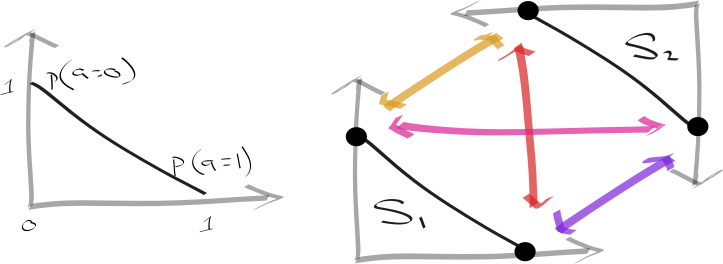
\includegraphics[width=1\textwidth,height=0.20\textheight]{../../pictures/drawings/2-state-2-action-simplices.png}
\caption{(left) Given that you are in state, $s$, we have a simplex over two actions $\{a_1, a_2\}$.
(right) The policy must describe distributions over actions for each state,
so the policy space must describe the $|S|$ possible combinations of distribution over actions.}
\end{figure}

\begin{figure}[h]
\centering
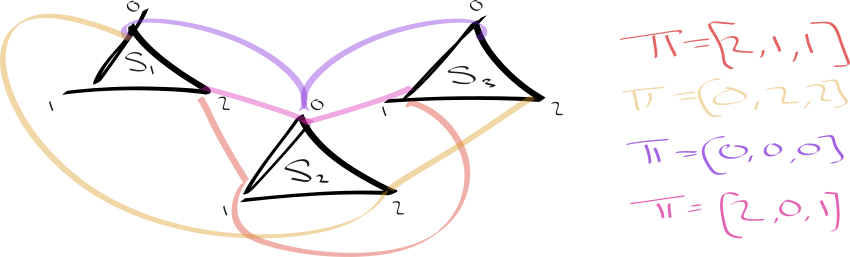
\includegraphics[width=1\textwidth,height=0.25\textheight]{../../pictures/drawings/3-state-3-action-simplices.png}
\caption{Here we are visualising the policy space of a three state, three action, MDP.
For each state, we must specify a distribution over actions.}
\end{figure}

\newpage

\section{Other properties of the polytope} \label{polytope-extras}



\subsection{Distribution of policies}

A potentially interesting question to ask about the value polytope is how the
values (of the policies) are distributed. we can calculate this
density analytically by using the probability chain rule:
\(p(f(x)) = \mid \det\frac{\partial f(x)}{\partial x}\mid^{-1}p(x)\).
Where we set \(f\) to be our value functional and \(p(x)\) to be a
uniform distribution over policies. Thus we have;

\begin{align}
p(V(\pi)) = |\det \frac{\partial V(\pi)}{\partial \pi}|^{-1} \cdot p(\pi) \tag{density}
\end{align}

\begin{figure}
\centering
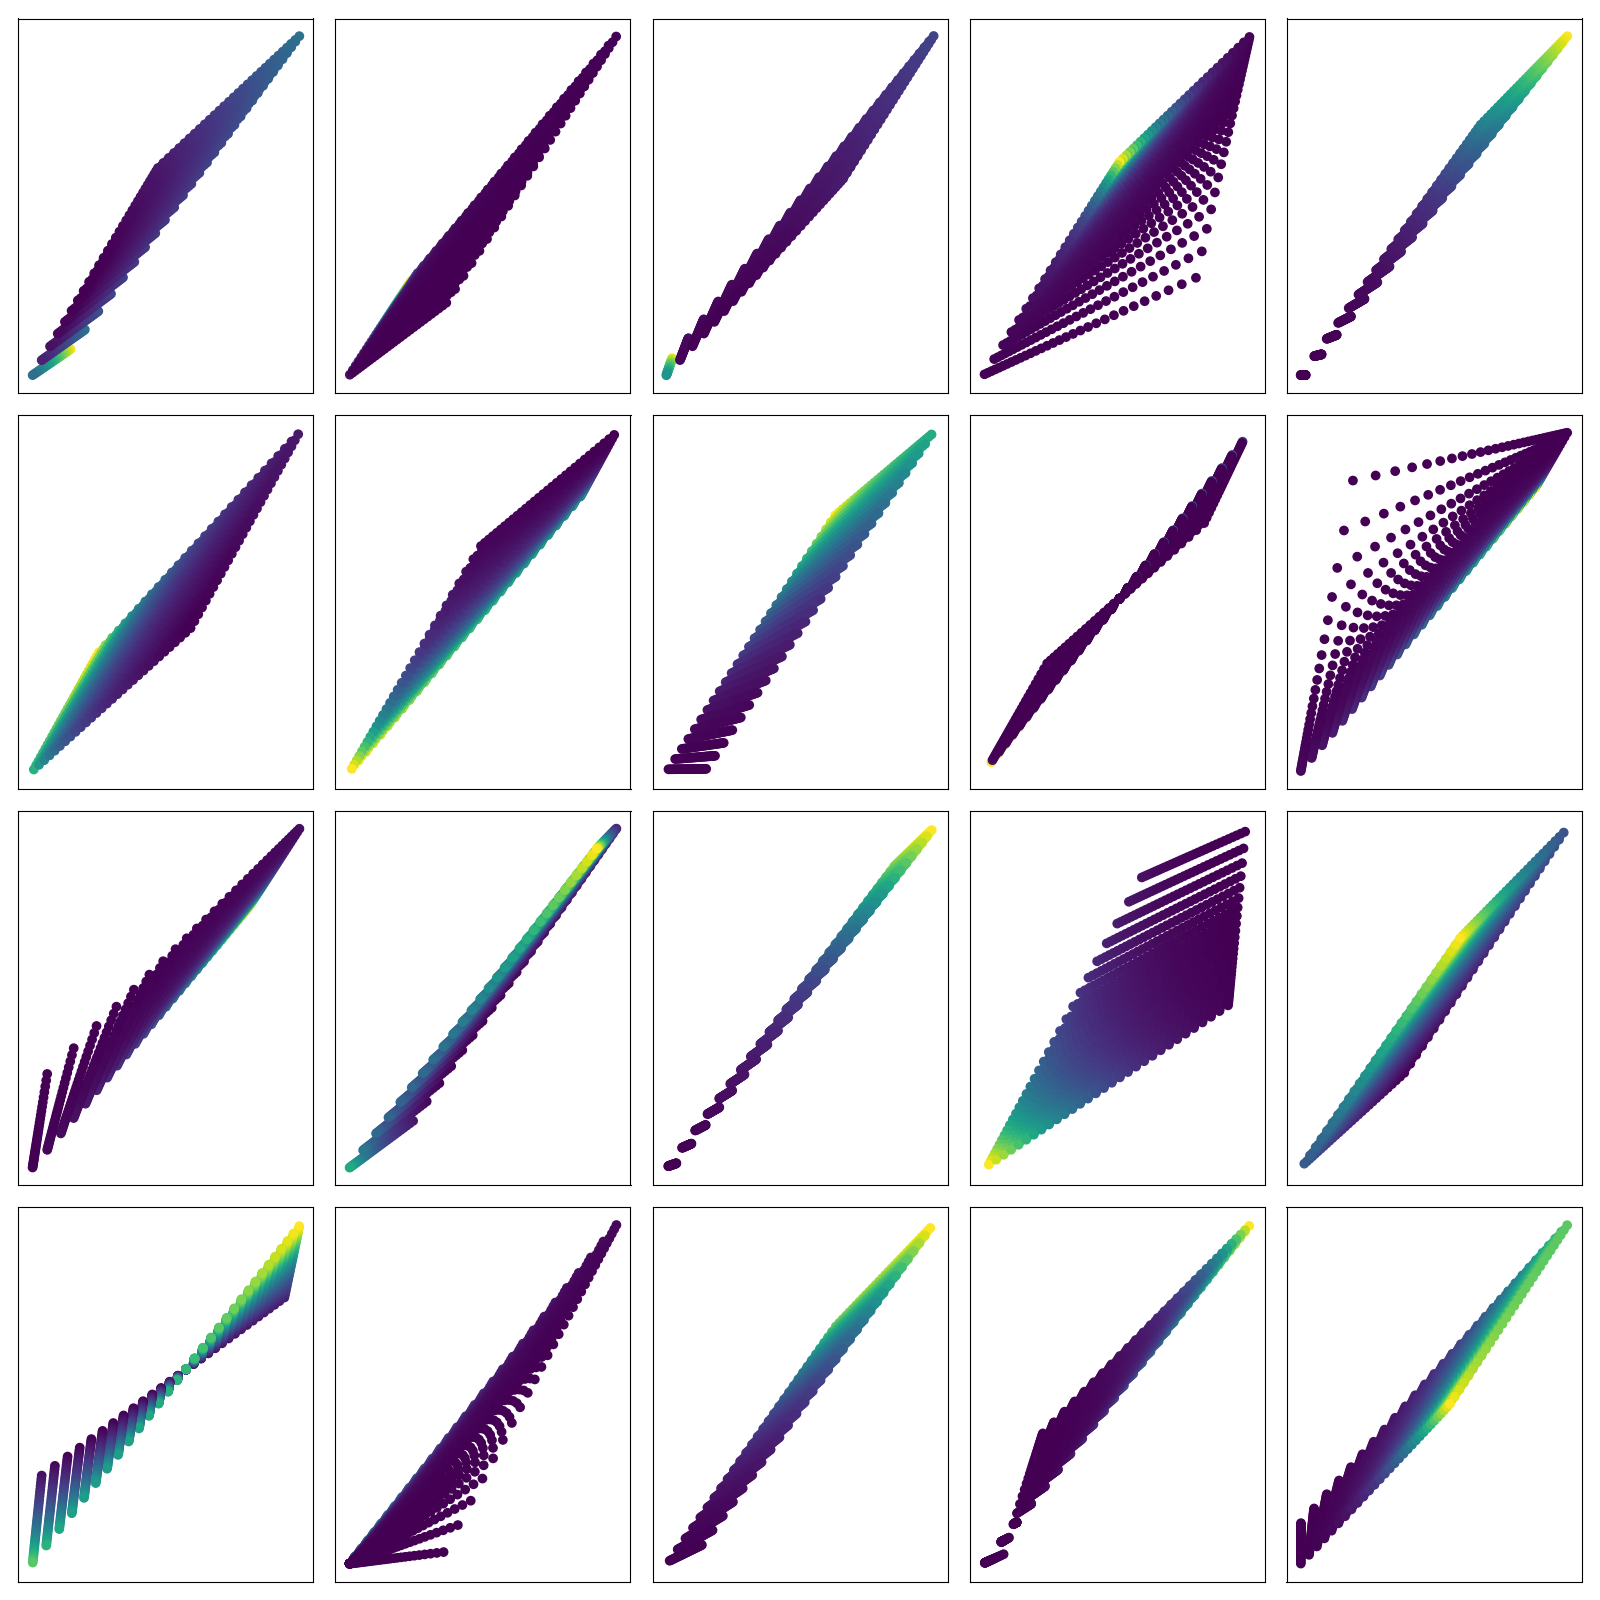
\includegraphics[width=1\textwidth,height=1\textheight]{../../pictures/figures/polytope_densities.png}
\caption{Here we have visualised the value polytope for 2-state 2-action MDPs. They are colored by the likelihood of
each value under a uniform distribution over policies.
Lighter color is higher probability.}
\label{fig:density}
\end{figure}

As we can see in \ref{fig:density}: for some polytopes, there is high density around the optimal policy.
In other polytopes, many of the policies are far away from the optimal policy.

Consider the expected suboptimality of our MDP, which tells us how far away the
optimal policy is from the 'center of value' of the polytope.

\begin{align*}
\mu_M(s) &:= \mathop{\mathbb E}_{\pi\sim\Pi}\Big[V_M^{\pi}(s) \Big]\\
\epsilon^{* }(M) &= \mathop{\text{max}}_s V_M^{\pi^{* }}(s) - \mu(M)(s)
\end{align*}

This suggests that MDPs with low expected suboptimality, $\epsilon^{* }(M)$, are easier to solve than other MDPs.
This is because we can simply sample a random policy which is likely to be close to the optimal policy
(or we could sample many policies and pick the best, which would, with high probability, be close(r) to the optimal policy).

\vspace{5mm}

\textbf{Open problem}\footnotemark[15]: If an MDP has sub-optimality,  $\epsilon^{* }(M)$,
then it is possible to find a $\epsilon$ optimal policy with $\{\}$ samples.

\footnotetext[15]{Open problem* of dubious interest.}

Where $\epsilon = \mathop{\text{max}}_s V^{\pi^{* }}(s) - V(s)$.

\vspace{5mm}

However, this strategy will not scale to higher dimensions.
As we increase the state size or action size, the chance that there is high
density near the optimal policy (or a randomly sampled MDP) decreases with rate proprtional to $|A|^{|S|}$.

% \textbf{Experiment:} Correlate the properties of \(P, r\) with entropy.
% Or find derivative wrt \(P, r\). What properties of \(P, r\) yield
% easily solvable MDPs?

\subsection{Discounting}

Another question you may have is: \textit{how does the shape of the polytope depend on the discount rate?}
Given an MDP, we can vary the discount rate from \(0\) to \(1\) and visualise
the shape of the value polytope.

\begin{figure}
\centering
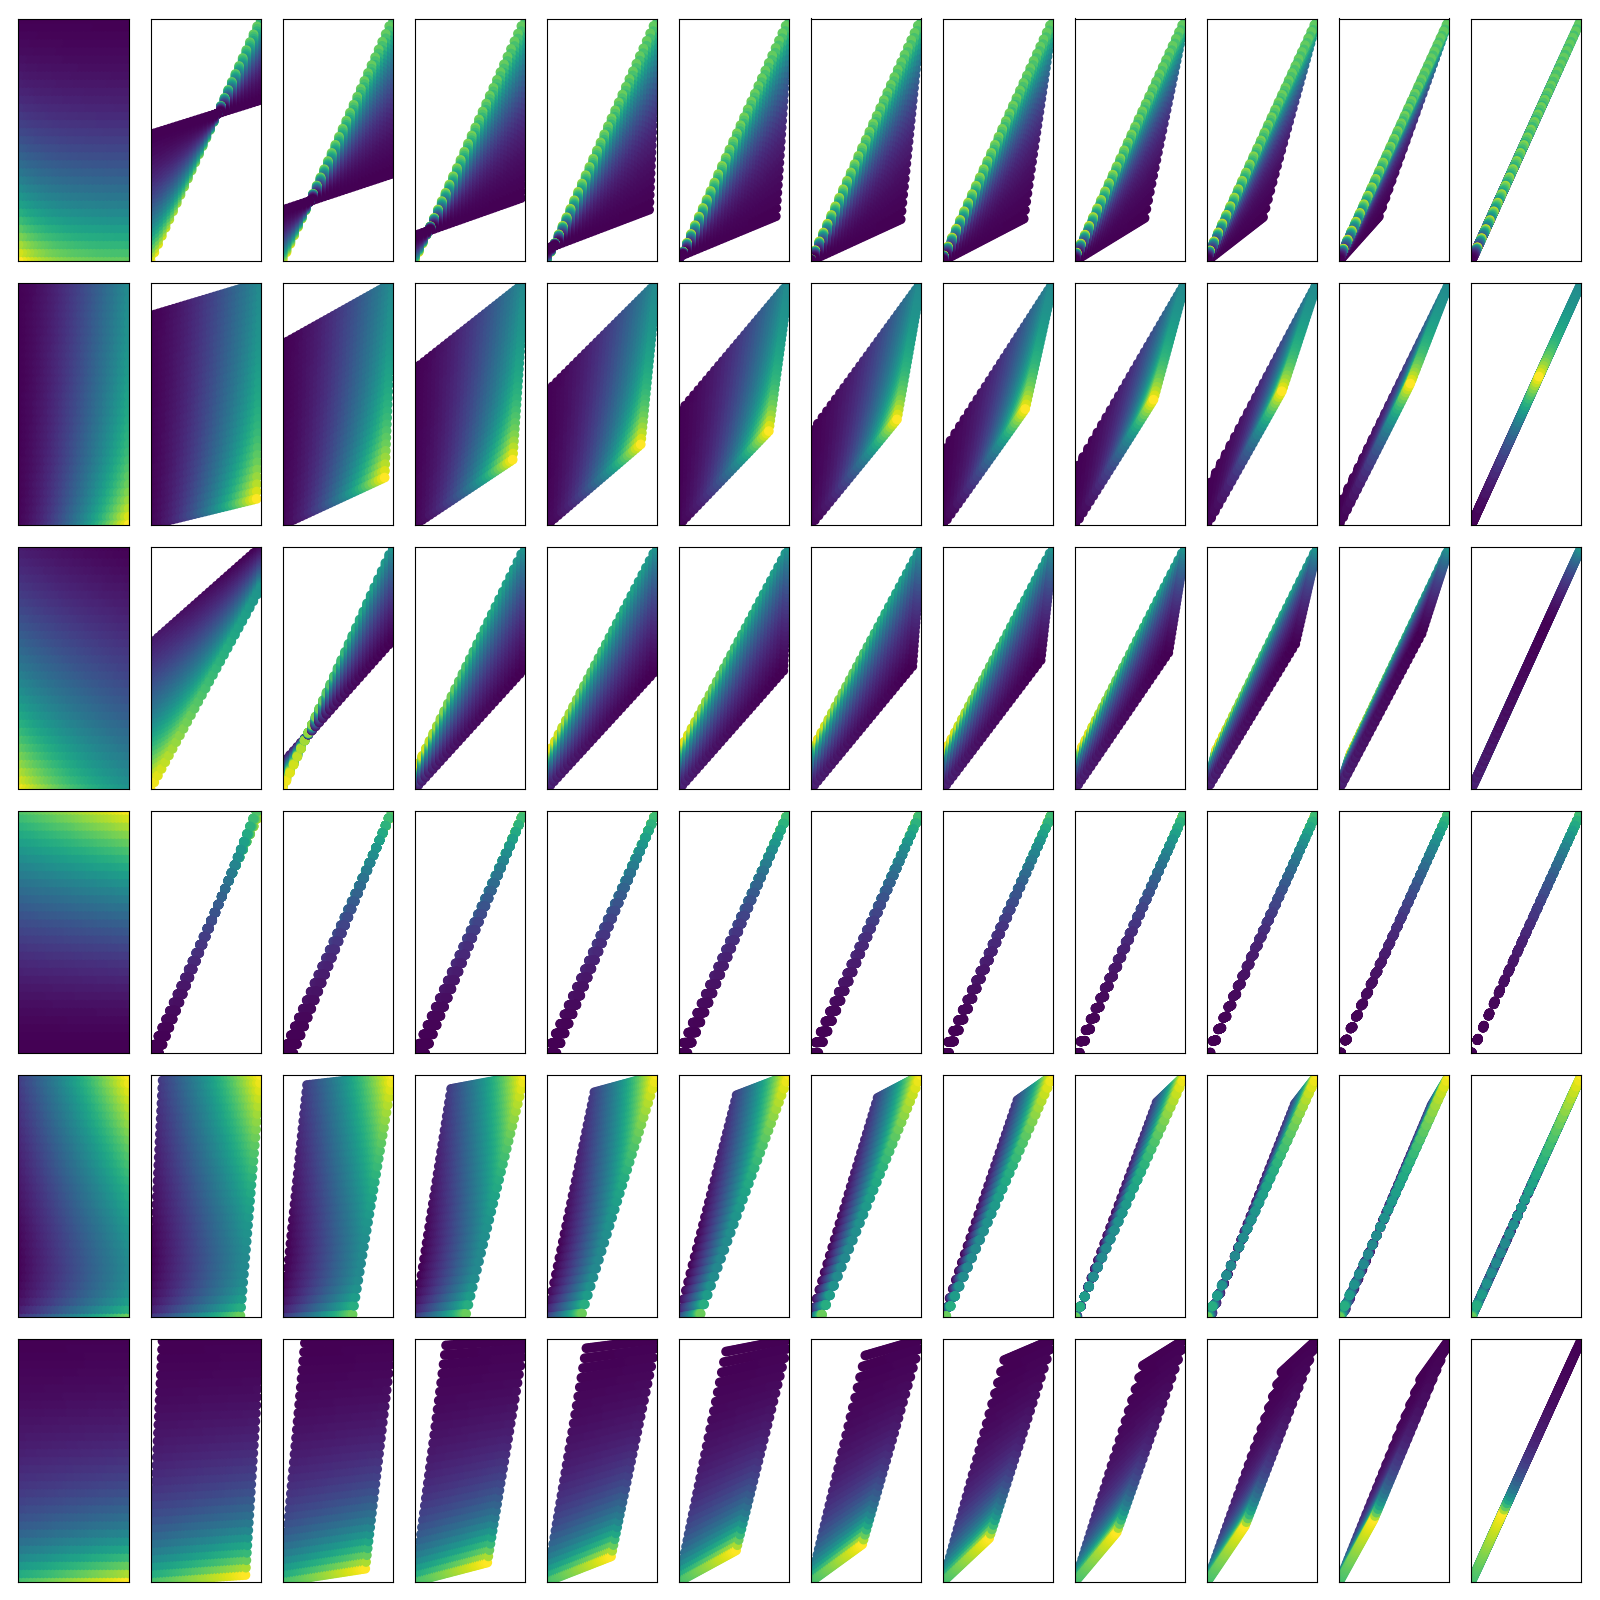
\includegraphics[width=1\textwidth,height=1\textheight]{../../pictures/figures/discounts.png}
\caption{Here we have visualised the value polytope for 2-state 2-action MDPs. The
rows show how their value polytopes change with changes in discount rate, ranging linearly from 0 (left), to 1 (right).
The color map is represents the density of policies, as in \ref{fig:density}.}
\label{fig:polytope-discounts}
\end{figure}

As we can see in \ref{fig:polytope-discounts}. As the discount rate tends to $1$,
all the policies are projected into a 1D space. (is this 1D for 2D problems. is it always 1D?)

\subsection{Derivation of derivative}

We want to derive the derivative of the value functional. Here we go.

\begin{align*}
V(\pi) &= (I − \gamma P_{\pi})^{−1}r_{\pi} \tag{value functional}\\
&= (I − \gamma P\cdot \pi)^{−1}r\cdot \pi \\
\frac{\partial V}{\partial \pi} &= \frac{\partial}{\partial \pi}((I-\gamma P_{\pi})^{-1} r_{\pi}) \\
&= (I-\gamma \pi P)^{-1} \frac{\partial \pi r}{\partial \pi}+   \frac{\partial (I-\gamma \pi P)^{-1}}{\partial \pi}\pi r\tag{product rule} \\
&= (I-\gamma \pi P)^{-1} r + -(I-\gamma \pi P)^{-2} \cdot -\gamma P\cdot \pi r\\
&= \frac{r}{I-\gamma \pi P} + \frac{ \gamma P\cdot \pi r}{(I-\gamma \pi P)^2} \tag{rewrite as fractions}\\
&= \frac{r(I-\gamma \pi P) + \gamma P \pi r}{(I-\gamma \pi P)^2} \tag{common demoninator}\\
& = \frac{r}{(I-\gamma P \pi)^2} \tag{cancel}
\end{align*}

\newpage
\section{Model search} \label{model-iteration}

As noted in \ref{search-spaces-mdps}, we can search through policy space or value
space, each with their own structure.
There is a third search space we could consider, the model parameters.

However, this problem is not a control problem like the search for values or policies.
This is an inference problem, we are trying to infer the model parameters.
Once we know these parameters, we can apply control.
In general, this is known as model-based RL.

We could search through models ($P, r$) using supervision from next step prediction.
This is a common approach to model-based RL \cite{Wang2019a}.
Rather, we consider using the value estimation error to guide the search for model parameters.

\begin{align}
\tilde P^{* }, \tilde r^{* } = \mathop{\text{argmin}}_{\tilde P, \tilde r} \int_{\Pi} \parallel V_{P, r}(\pi)-V_{\tilde P, \tilde r}(\pi) \parallel_\infty
\end{align}

\begin{figure}
\centering
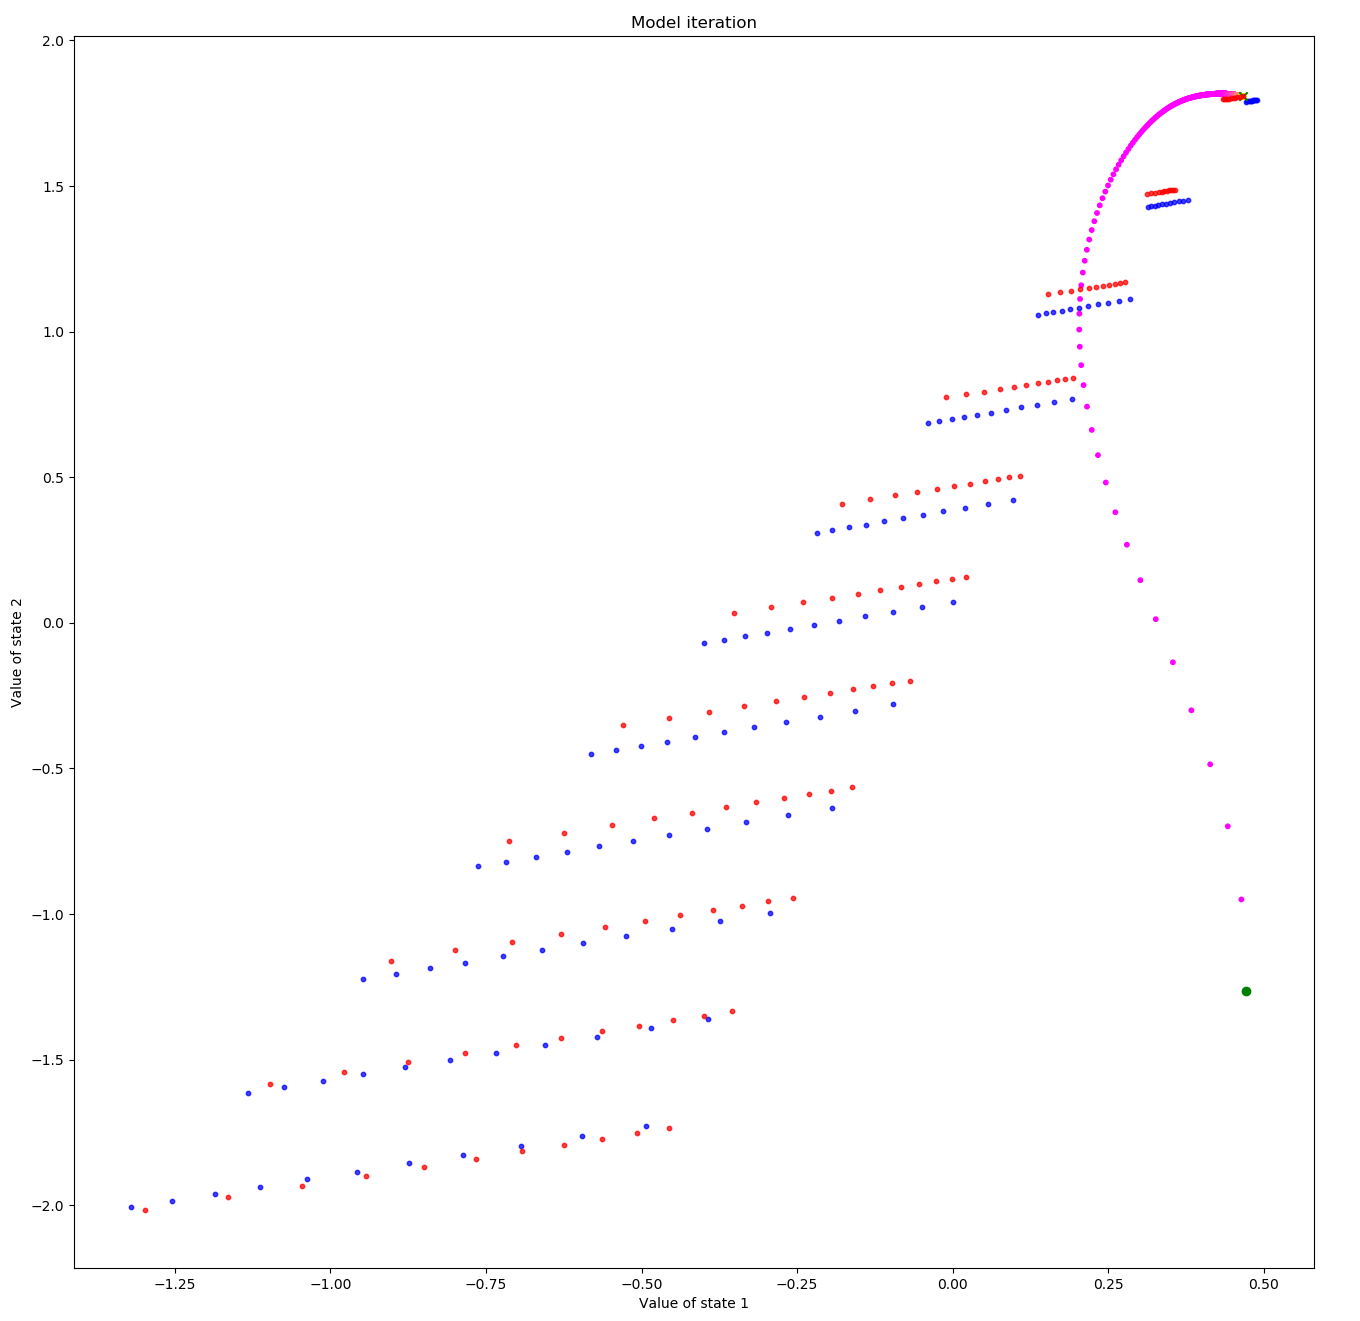
\includegraphics[width=1.0\textwidth,height=0.8\textheight]{../../pictures/figures/model_iteration.png}
\caption{Model iteration applied to a 2-state, 2-action MDP.
Blue shows the value of policies when evaluated under the true model, $P, r$,
and Red shows the estimated value of policies when evaluated under the learned model at convergence, $\tilde P, \tilde r$.}
\end{figure}

There is a main advantage and some disadvantages to this framework.
The advantage is that this approach focuses its resources only on 'relevant' features of the model.
The disadvantages are that it requires many policy evaluations (from the environment),
and many estimates of a policy's value (simulated evaluations).

\subsection{Relevant features of the model}

Model iteration via value prediction error only focuses on 'relevant' features of the model \footnotemark[31].
Relevant in the sense that they are useful for accurately predicting state values.

\footnotetext[31]{Model free approaches to RL also focus on 'relevant' features, however, they do not explicitly represent the underying model.}

Consider a problem where the reward is only determined by the first feature of the state.
We can add arbitrarily many extra features. A model-based learner that learns through next step prediction will attempt to
accurately predict all of these features. This unnecessarily spends resources.

More formally; let the state space but a subset of the reals $S \subset \mathbb R^d$.
And construct a reward function that is only dependent on the first feature of the state space, $r(s, a) = f(s^0, a)$.
While the transition function is constructed so that, there exists a $k$ dimensional subspace (that includes the first feature)
that is independent of the other $d-k$ features, $P(s'|s, a) = [g_1(s^{0:k}, a), g_2(s^{k:d}, a)]$.

An example with this structure, could be the addition of $d-k$ 'noise' features,
that play no part in the transition dynamics, but only describe inessential features
(such as features that describe the positions of leaves on a windy day).

% \subsection{Jokes}
%
% This is just a less intelligent reinvention of Thompson sampling for MDPs.
% No it isnt?!? They use

\subsection{Policy evaluations}

We receive $V_{P, r}(\pi)$ from the environment. But we want to minimise the number
of these calls to the environment, as it can be expensive to evaluate a policy with high accuracy.

Also, for each iteration of $\tilde P_t, \tilde r_t$, we need to estimate the
value of many policies, $\forall \pi; V_{\tilde P_t, \tilde r_t}(\pi)$. This requires lots of compute.

Rather than integrating over all policies (thus requiring us to evaluate all of them),
we only need the deterministic policies. As, Bellamare et al. 2019 show that \textit{"the maximal approximation error
measured over all value functions is the same as the error measured over the set of extremal vertices [aka deterministic policies]"}\cite{Bellemare2019b}.
However, this still requires us to evaluate $|A|^{|S|}$ policies, and to simulate $T |A|^{|S|}$ policies. \footnotemark[32]

% maybe a connction to compressed sensing?!
\footnotetext[32]{It should be possible to use off policy estimation techniques to further reduce the required samples / compute. But we leave this for future work.}

\newpage
\section{Visualising higher dimensional MDPs}\label{graph-vis}

So this value polytope works well for 2D. And could be extended to 3D. But, what about higher dimensions?

\begin{displayquote}
  \textit{"To deal with a 14-dimensional space, visualize a 3-D space and say 'fourteen' to yourself very loudly. Everyone does it."} Geoff Hinton
\end{displayquote}

Is there intuition we might gain from visualising optimisation on MDPs with the
number of states and / or actions being greater than 3?

How to construct them? Decompose the value of a policy as a convex combination
of the values of the deterministic policies.

\begin{align*}
  \alpha(\pi) = \mathop{\text{argmin}}_{\alpha \in \Delta^n} \parallel  V(\pi) - \sum_i (V(\pi_i) \cdot \alpha_i ) \parallel_2^2 + H(\alpha)
\end{align*}

The entropy term ensures we prefer convex combinations with lower entropy.
% Properties of the graphs / graph signals?
\newpage

\begin{figure}[!h]
\centering
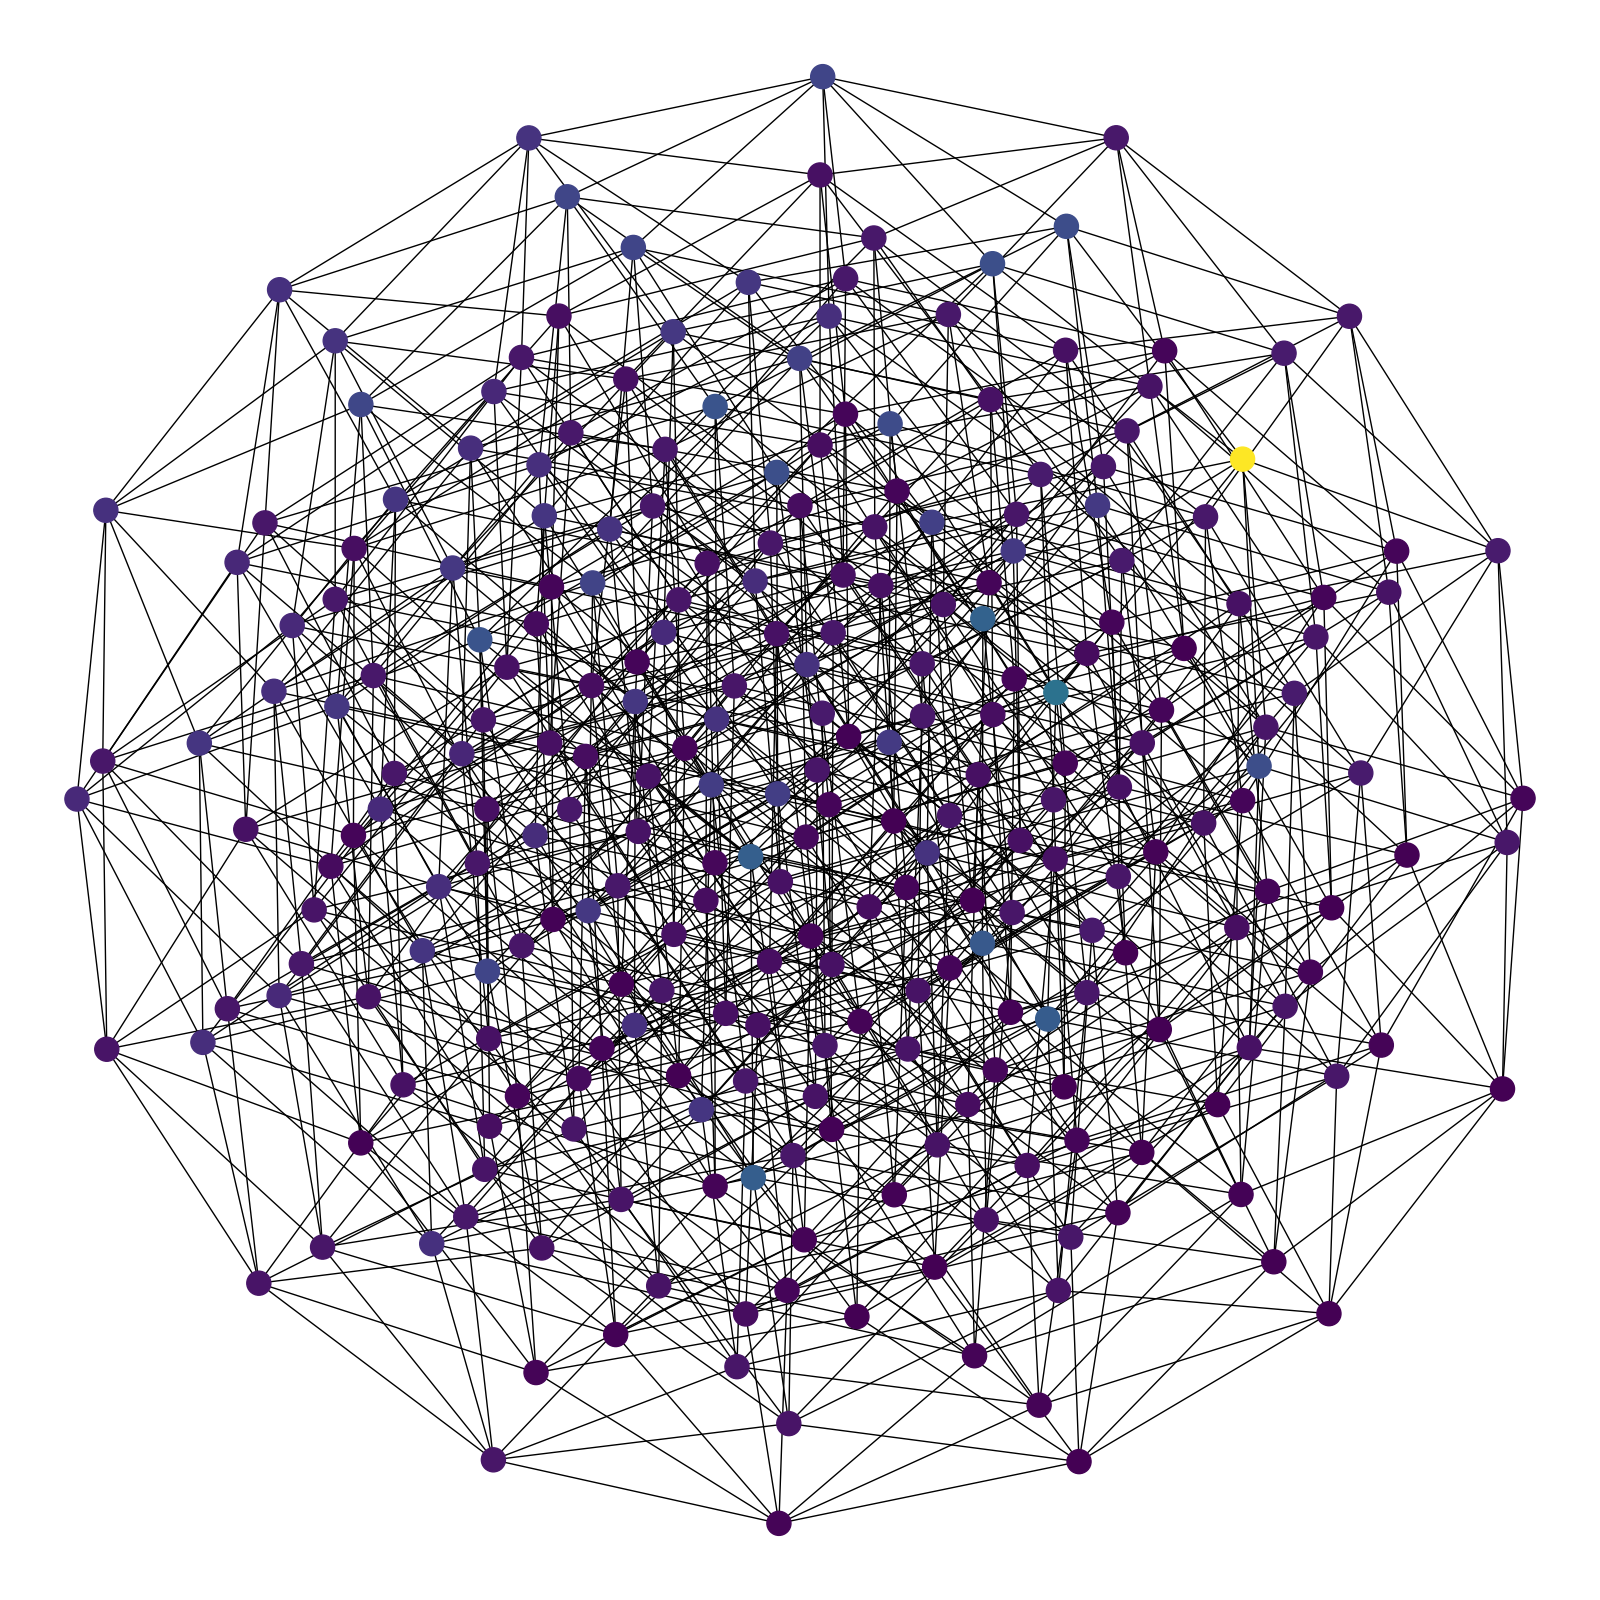
\includegraphics[width=0.5\textwidth,height=0.3\textheight]{../../pictures/figures/discrete-graph.png}
\caption{PI bounces between the nodes of the graph.
So the search of the optimal policy using PI can be visualised as the walk along a graph.
Note: the current policy is shown in yellow (close to the top right).}
\end{figure}

% As each node is a deterministic policy.
% Thus policy iteration is equivalent to finding the shortest path on a XX connected policy graph.

\begin{figure}[!h]
\centering
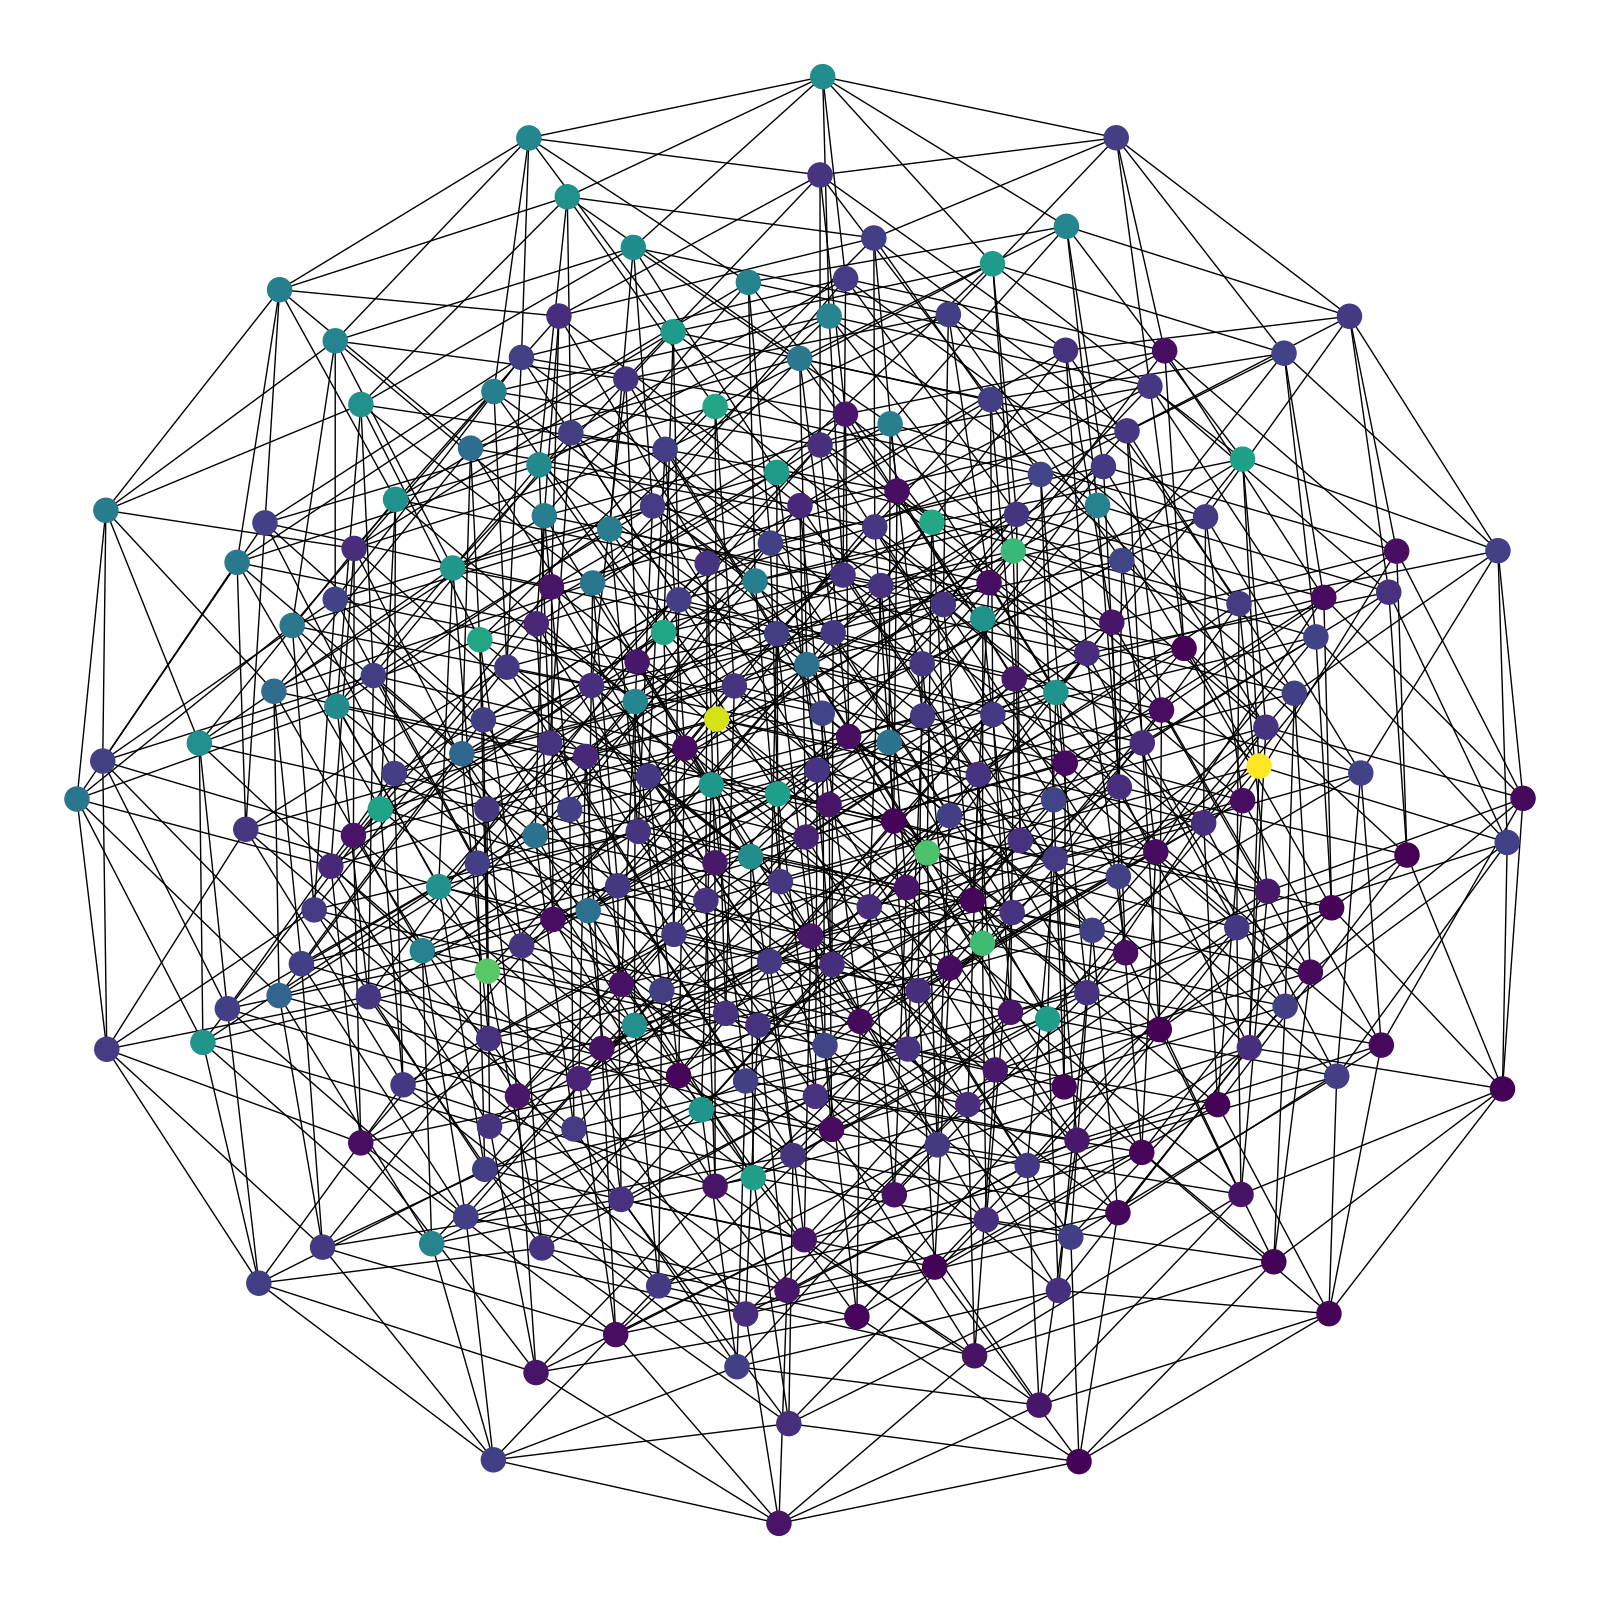
\includegraphics[width=0.5\textwidth,height=0.3\textheight]{../../pictures/figures/interior-graph.png}
\caption{Policy gradient traverses through non-deterministic policies.
So the search of the optimal policy using PG can be visualised the dynamics of a graph signal.}
\end{figure}


\newpage
\section{Deep policy gradients}\label{ss-extras}

From the search spaces section \ref{search-spaces-mdps}, we are left wondering;

\begin{itemize}
\tightlist
\item In which spaces can we (efficiently) calculate gradients?
\item In which spaces can we do convex optimisation?
\item In which spaces does momentum work (well)?
\end{itemize}

Currently, the most successful deep RL approaches are variants of policy gradient methods \cite{Mnih2016,Schulmanb}.
Despite their efficacy in practice, we still don't have a good understanding of
how policy gradient methods combine with deep learning methods to give performant agents.

A key feature of deep learning is over parameterisation (among the other features;
hierarchies, non-linearity, smoothness, locality). There has been recent work
attempting to understand the effect of overparameterisation \cite{Arora2018}.

Here we explore the effects of;
\begin{itemize}
\tightlist
  \item overparameterising the policy and then using policy gradient methods to find the optimally policy.
  \item reparameterising the loss function, thus yielding some ither space to search through.
\end{itemize}

% \begin{figure}[!h]
% \centering
% 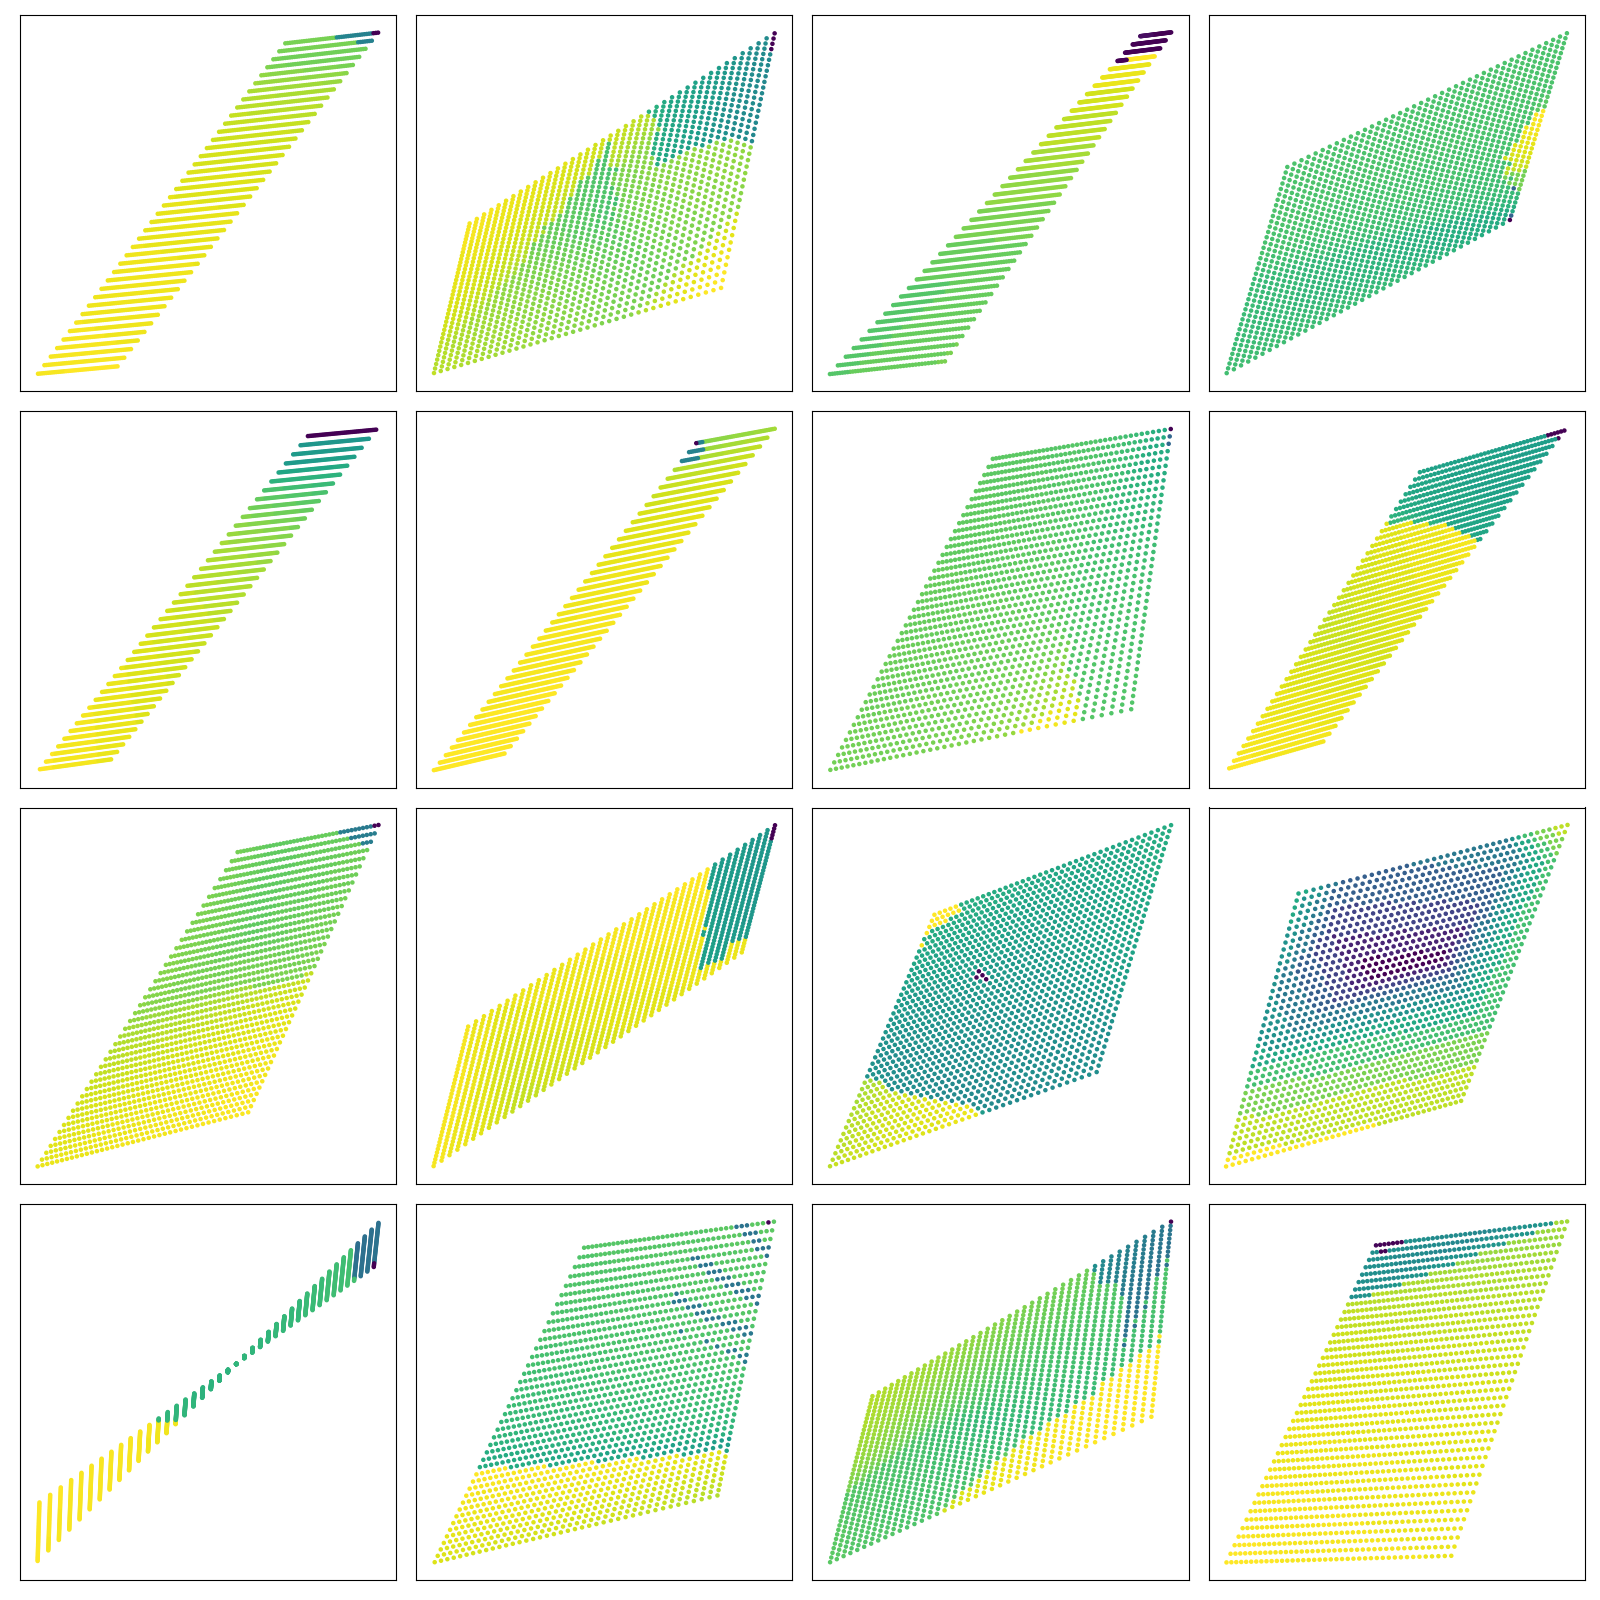
\includegraphics[width=1\textwidth,height=1\textheight]{../../pictures/figures/mvi-iterations.png}
% \caption{Above you see: various MDPs where the value of each policy is colored
% by the number of iterations it took to converge to the optimum policy. Yellow is many iterations, purple is few iterations.}
% \end{figure}


% {\color{red}TODO. need to include some plots of vanilla PG}

\subsection{Overparameterisation}

Recently there has been work investigating the properties of overparameterised search spaces.
Arora et al. 2018 \cite{Arora2018} prove that overparameterisation yields acceleration, however,
their explanation of the acceleration is not entirely convincing (as it requires first order assumptions).

More applied to RL, we want to know: how does overparameterisation effect the search for optimal policies?

In figures \ref{fig:param-compare-sgd} and \ref{fig:param-compare-sgd} we can see that
parameterisation can yield vastly different training trajectories to gradient descent,
{\color{red}and it's relation to momentum?!}\footnotemark[33].

\footnotetext[33]{It is important to remember that these trajectories also reflect exploration.
It seems interesting to ask, if there are any advantages to certain types of trajectory?}

{\color{red}TODO regenerate these figures. better quality.}

\begin{figure}
\label{fig:param-compare-sgd}
\centering
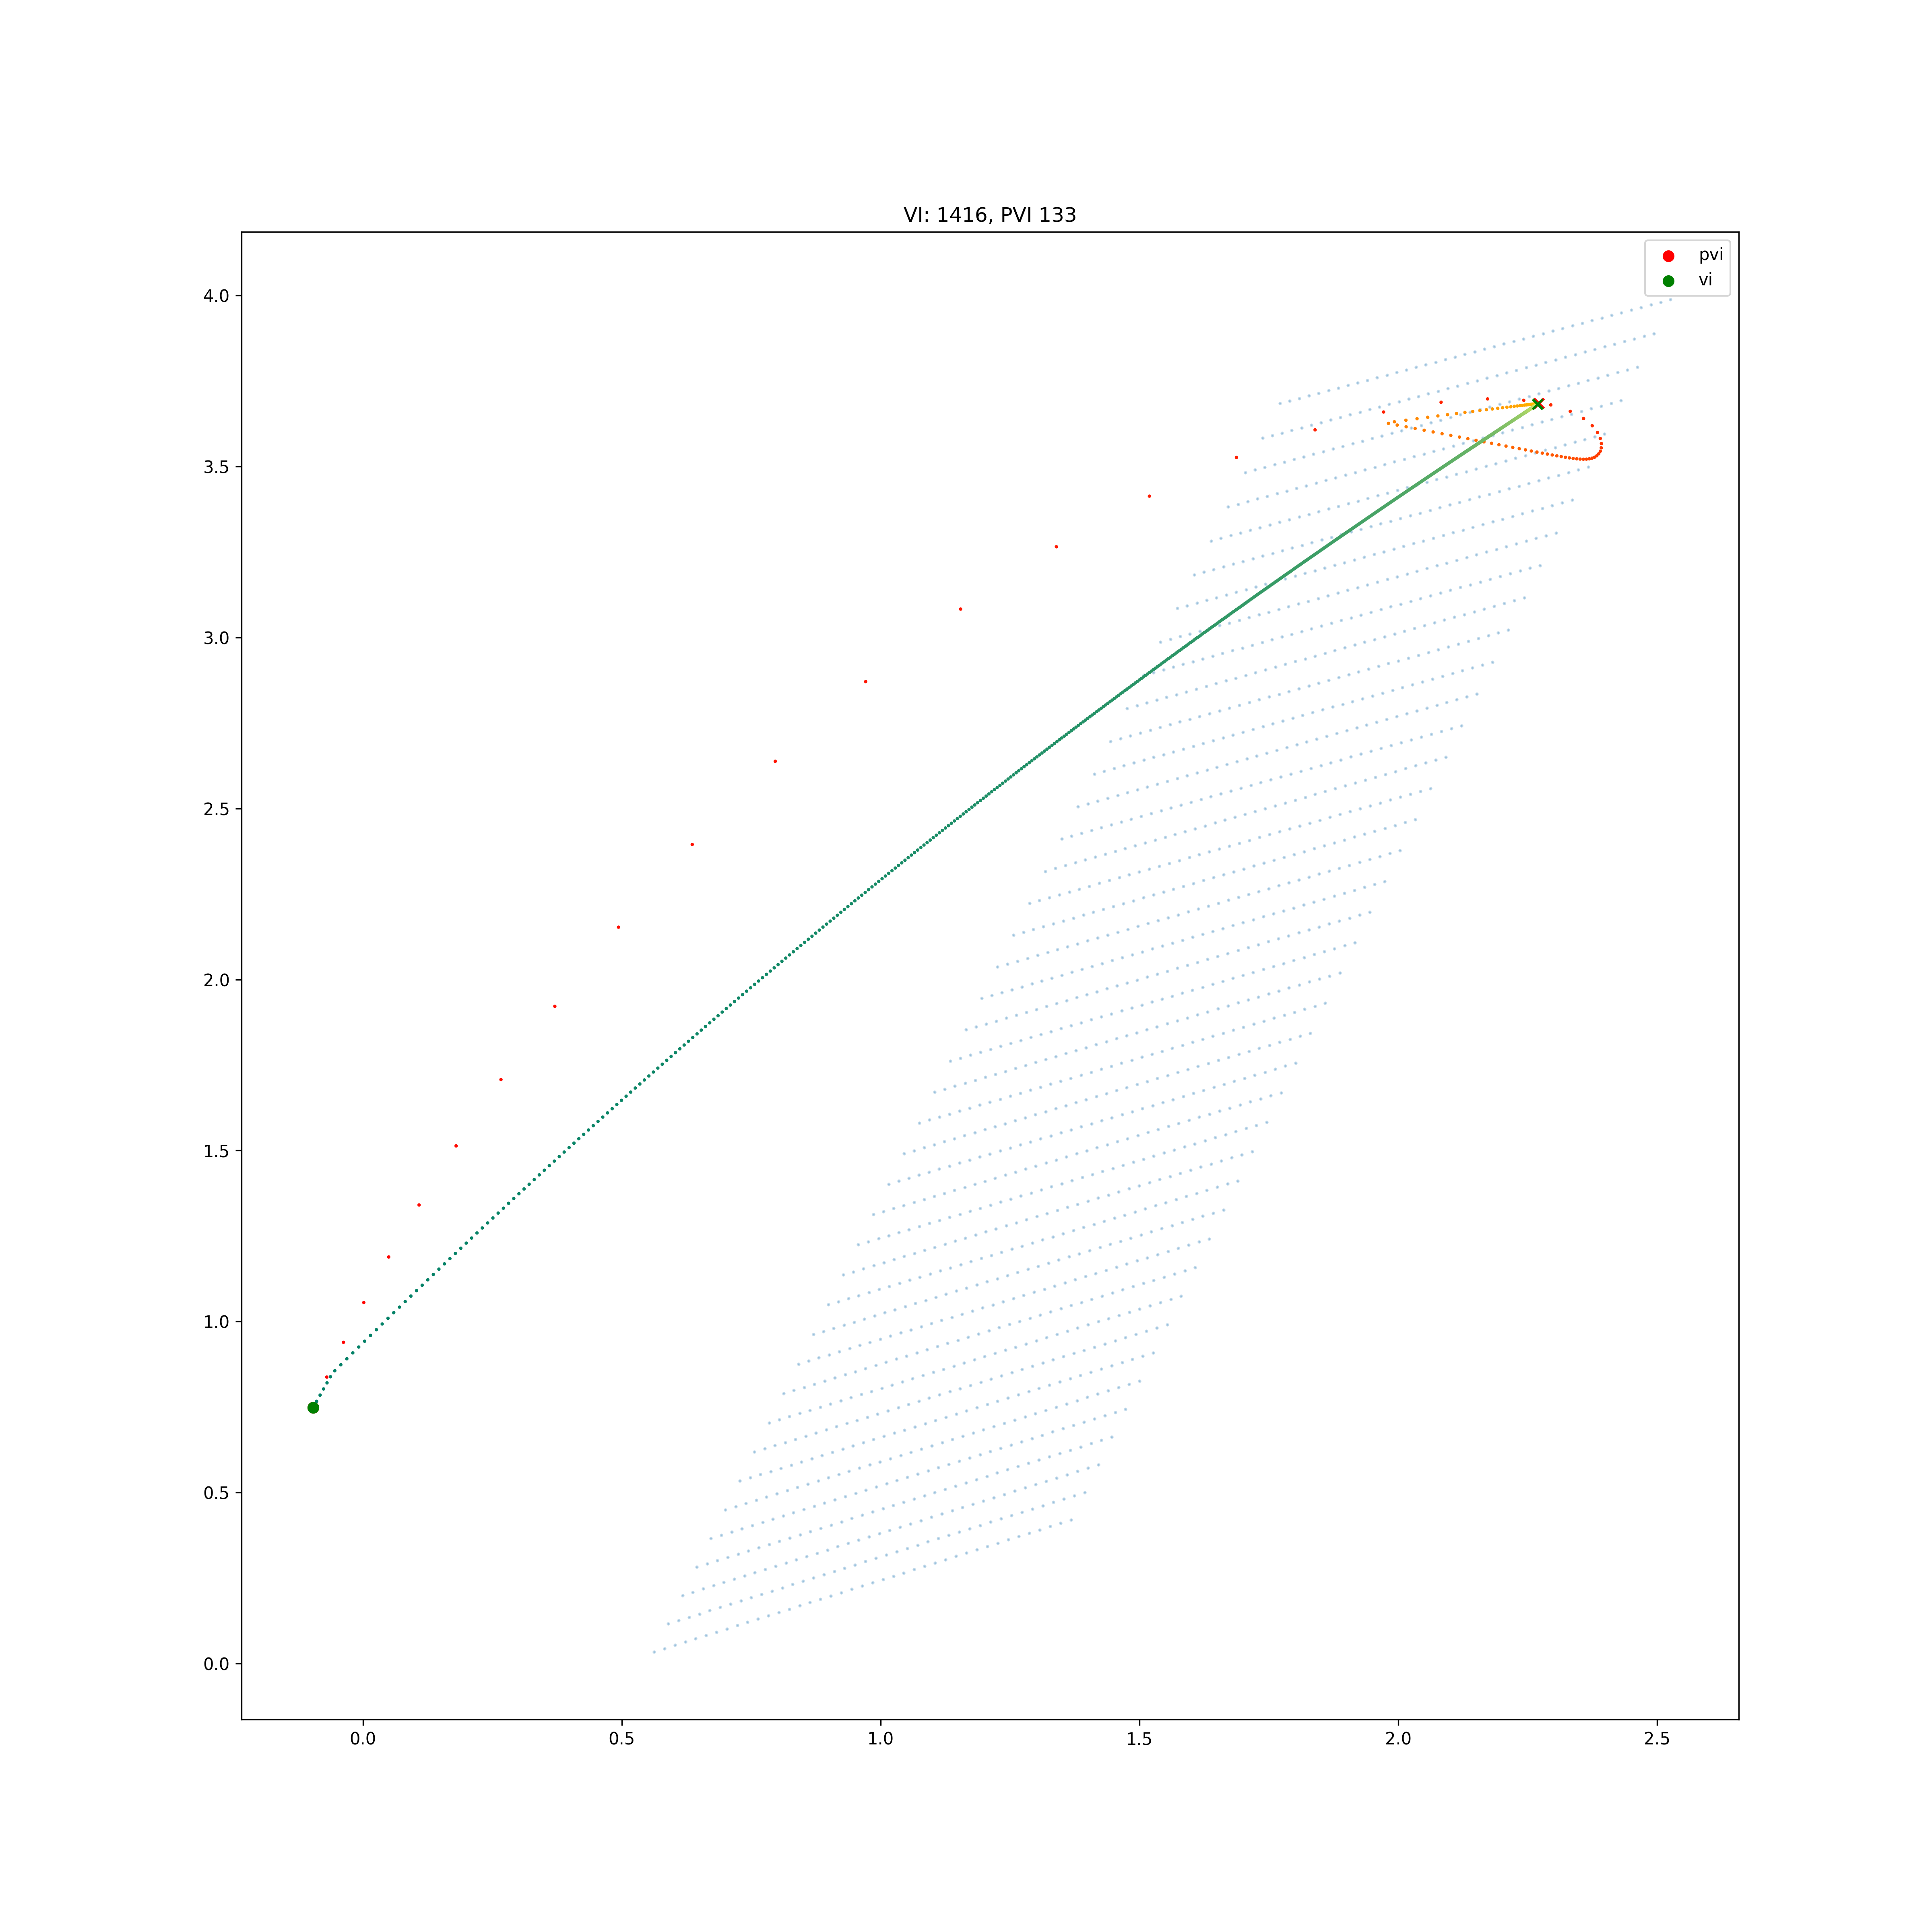
\includegraphics[width=1.0\textwidth,height=0.5\textheight]{../../pictures/figures/vi-vs-pvi.png}
\caption{The optimisation dynamics of value iteration versus parameterised value iteration.}
\end{figure}

\begin{figure}
\label{fig:mom-compare-sgd}
\centering
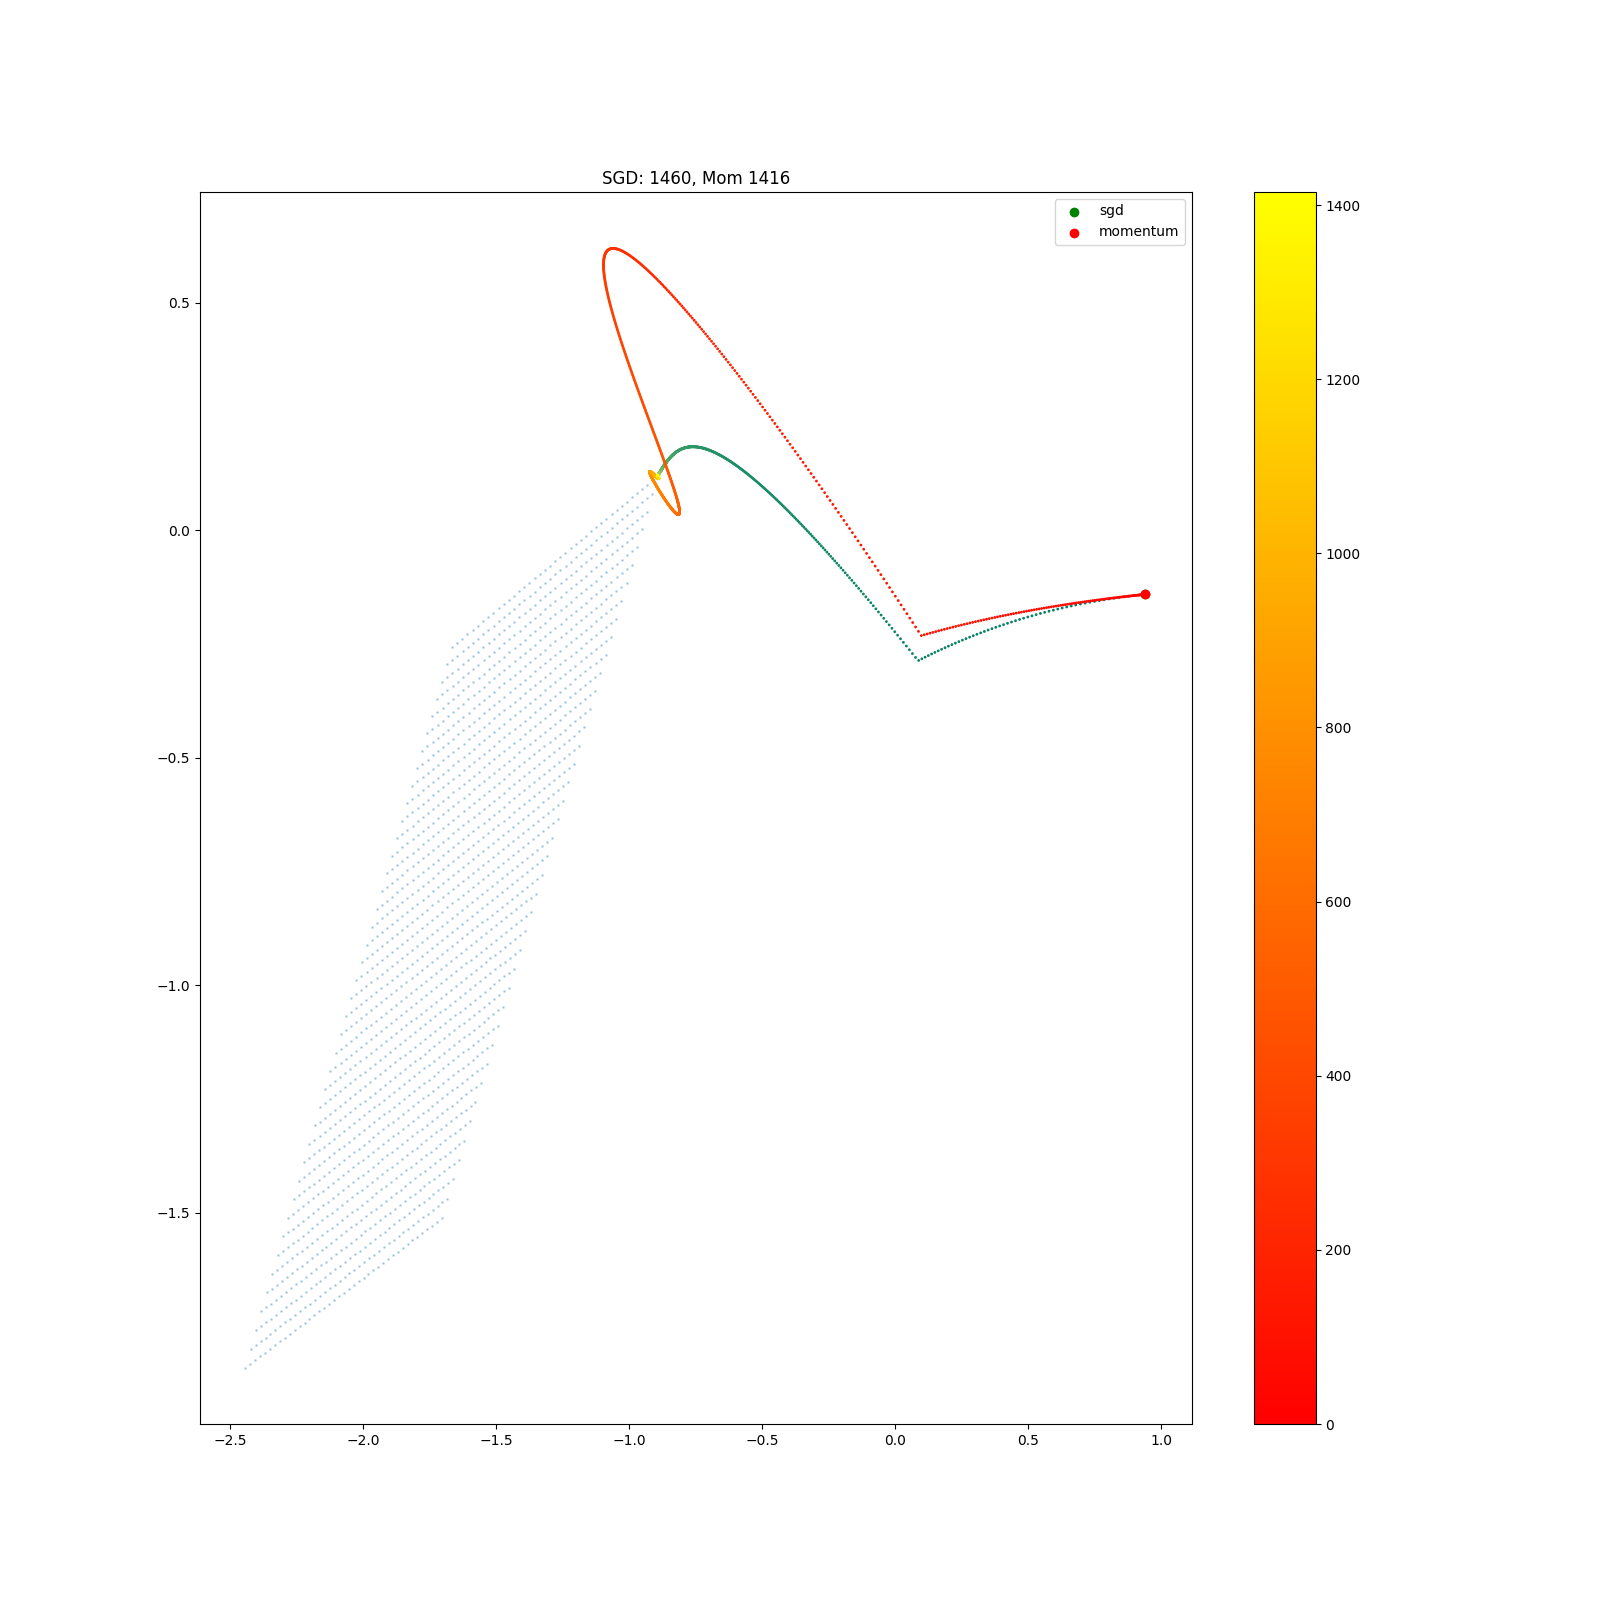
\includegraphics[width=1.0\textwidth,height=0.5\textheight]{../../pictures/figures/vi_sgd-vs-vi_mom.png}
\caption{The optimisation dynamics of value iteration versus value iteration with momentum.}
\end{figure}

{\color{red}Also. Have some more of the ims below coming}

In \ref{fig:iteration-complexity} we can observe that there can be sharp boundaries
between neighboring policies. A kind of phase transition, between the optimal policy being easy to find, and not.
(despite the fact that the we started from neighboring points).

\begin{figure}
\label{fig:iteration-complexity}
\centering
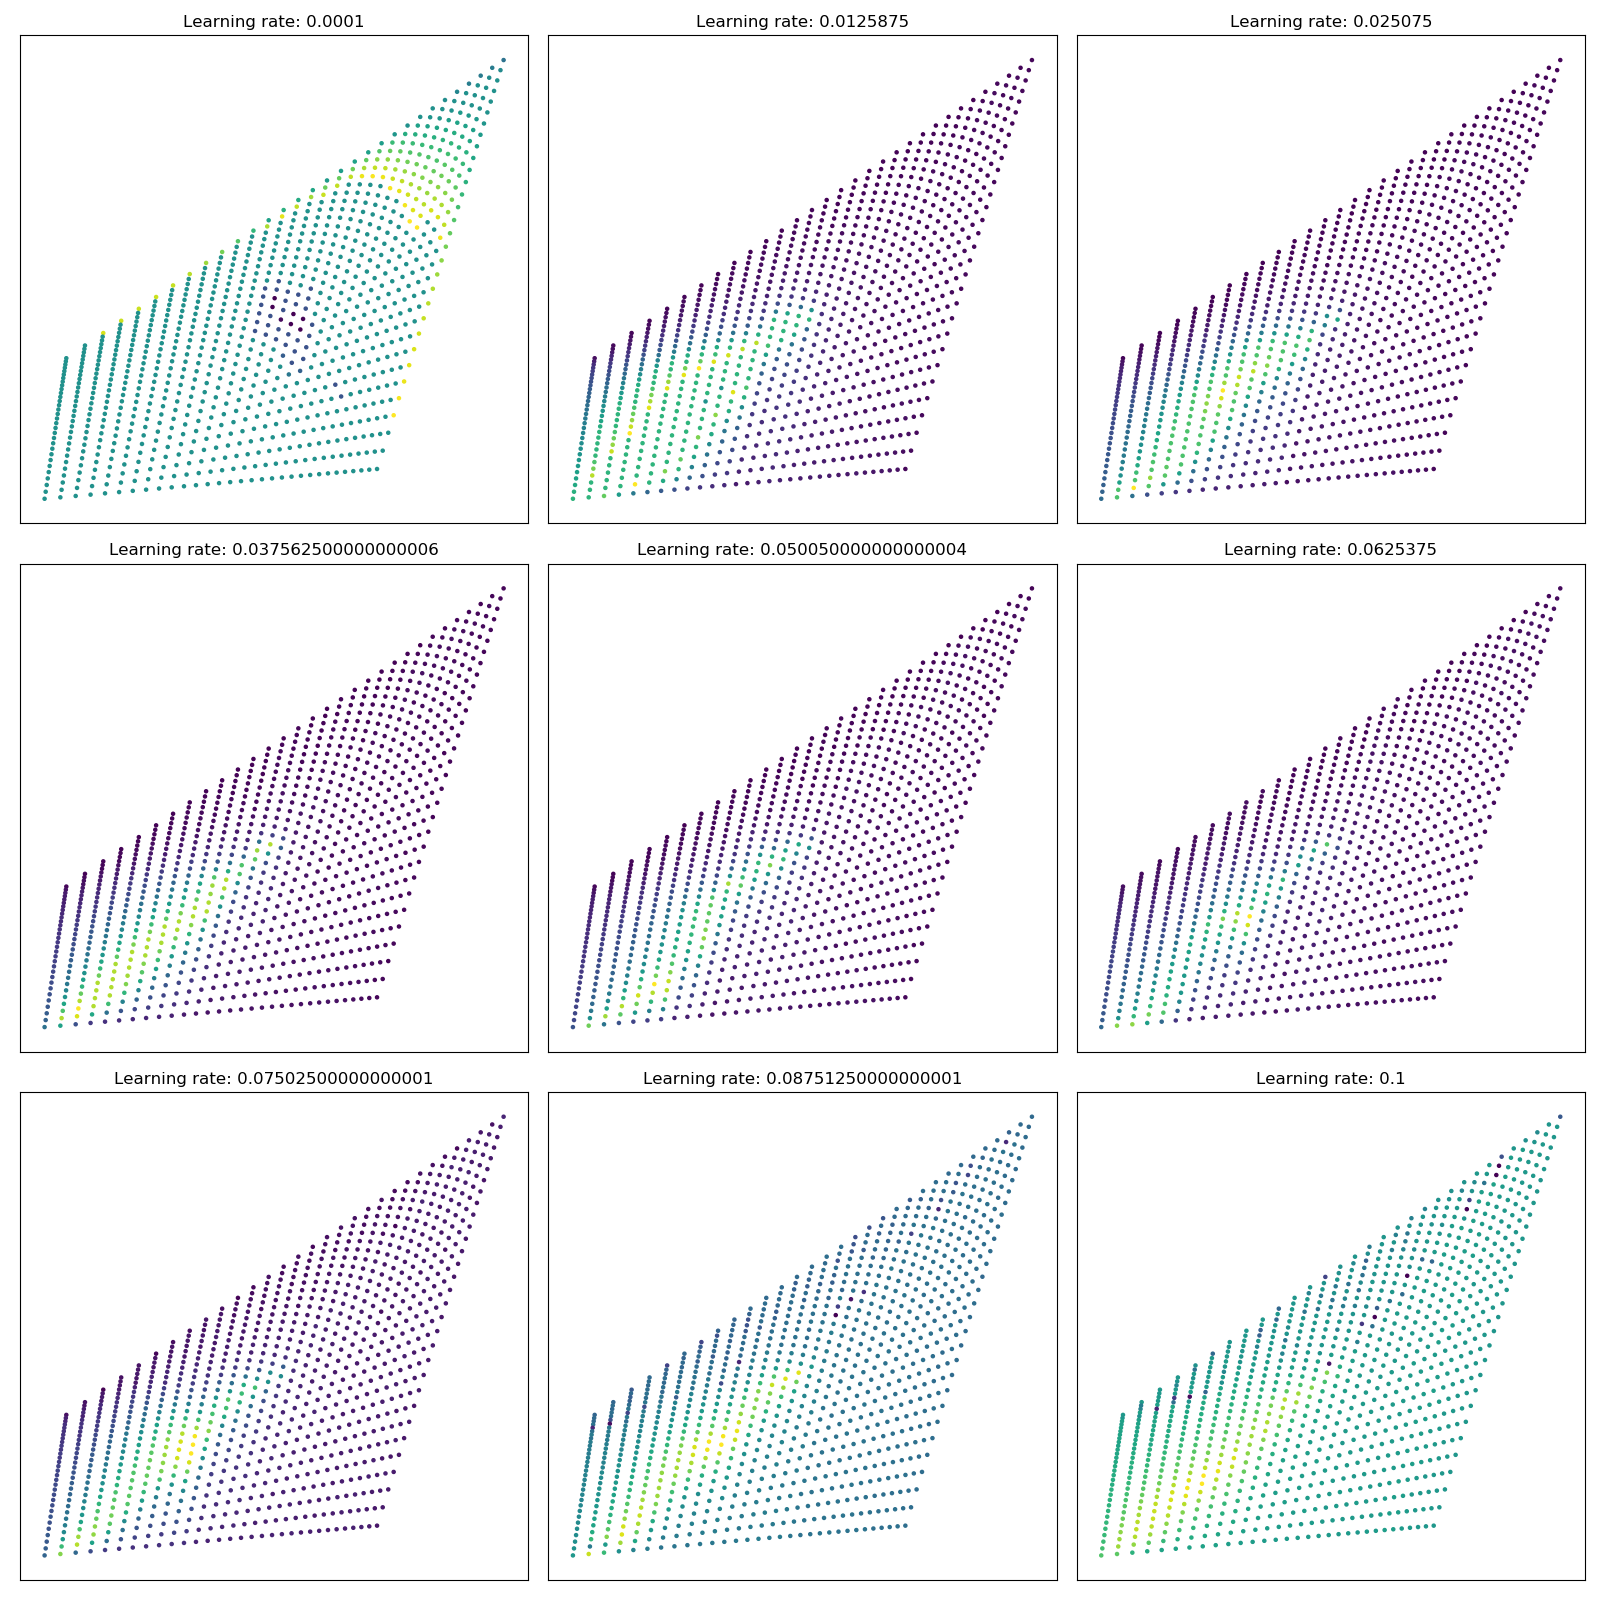
\includegraphics[width=1.0\textwidth,height=1.0\textheight]{../../pictures/figures/iteration-lr-0.png}
\caption{Here we have visualised the value polytope a 2-state, 2-action MDP.
These value polytopes are colored by the iteration complexity (many iterations - yellow, few iterations - purple) of parameterised policy gradients.
Each polytope was generated using a different learning rates.}
\end{figure}


% In which spaces can we get the most information? (e.g. low variance gradients)
% In which spaces to we have access to reliable guidance (e.g. large magnitude gradients)?
% SNR

% \cite{Brandfonbrener2019} consider the same setting, with an additional simplification. In the cts limit. No step sizes / learning rate.
% Obviously this simplification is not realistic. As in our experiments we see divergence with a overparameterised linear model.

% If we overparameterise the search space, then we can move between solutions in new ways. We can `tunnel' from A to B, without crossing C.
%  insert pic / prove
%
% Every point (in output space) is closer, when measured in the distance in parameter space needed to be traveled.
% insert pic / prove

\newpage
\section{Reparameterisation}

% Its effect on topology and acceleration.

{\color{red}Not sure if I should include this section. Very early stage...}

\begin{displayquote}
  \textsl{If we are allowed to arbitrarily pick our optimisation space, which should we pick?}
\end{displayquote}

Here we raise the question: should, and if so, how can, we rationally pick the
search space given knowledge of the loss function and likely starting points?

Consider the simple convex problem;

\begin{align*}
  x^{* } = \mathop{\text{argmin}}_{x} x^2
\end{align*}

We can pick some other space, $Z$, that we want to search in. And we can map $Z$ on to $X$ using $f: Z \to X$.

\begin{align*}
  z^{* } &=\mathop{\text{argmin}}_{z} f(z)^2 \\
    x^{* } &= f(z^{* })
\end{align*}

If we pick some simple functions for $f$. What happens? Well, if $f$ is non-linear
then we lose the guarantees convergence of convex search. However, what is gained?

\begin{figure}[h!]
\centering
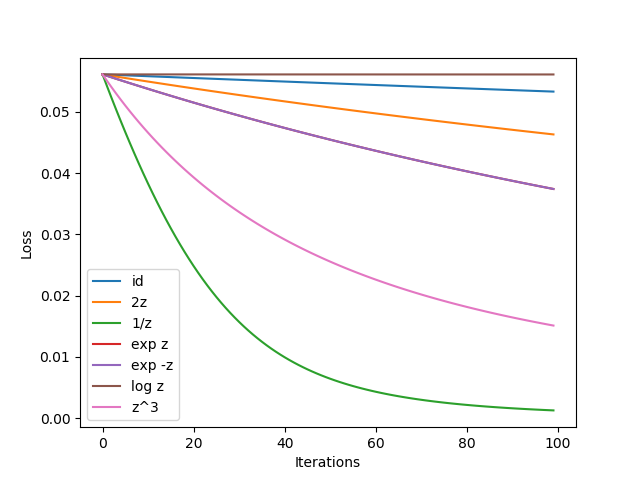
\includegraphics[width=0.7\textwidth,height=0.35\textheight]{../../pictures/figures/reparam-ce-04.png}
\caption{The iteration complexity of different initialisations and different learning rates.}
\end{figure}

\begin{figure}[h!]
\centering
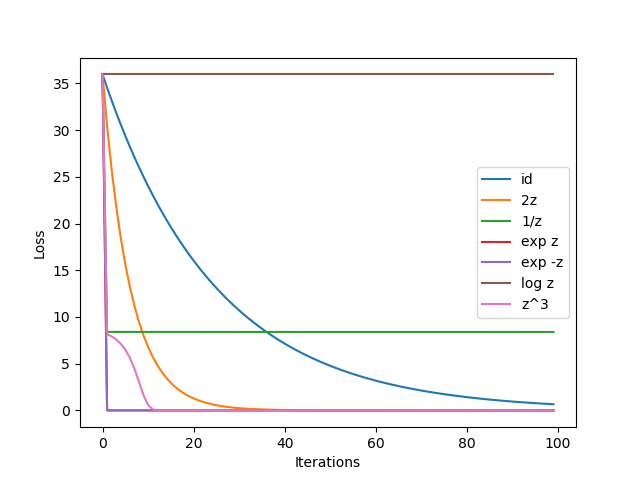
\includegraphics[width=0.7\textwidth,height=0.35\textheight]{../../pictures/figures/reparam-mse-04.png}
\caption{The iteration complexity of different initialisations and different learning rates.}
\end{figure}

When $z$ is the parameters of a deep neural network, the search space has certain properties: for example it's euclidean.
An alternative could be to search through a hyperbolic space, yielding 'hyperbolic neural networks' (explored by \ref{Ganea2018}).
